%!TEX root = ../template.tex
%%%%%%%%%%%%%%%%%%%%%%%%%%%%%%%%%%%%%%%%%%%%%%%%%%%%%%%%%%%%%%%%%%%
%% chapter1.tex
%% NOVA thesis document file
%%
%% Chapter with introduction
%%%%%%%%%%%%%%%%%%%%%%%%%%%%%%%%%%%%%%%%%%%%%%%%%%%%%%%%%%%%%%%%%%%

%Introdução 3-5
%Enquadramento
%Motivação
%Proposta de trabalho

\typeout{NT FILE chapter1.tex}%

\chapter{Introduction}
\label{cha:introduction}

The world is always looking for newer and better ways to improve efficiency and durability of everything including ourselves. Wearable technology is an example of this research and its popularity is increasing over time. 
These devices have a great wide-range of functions that can help in medical diagnosis, injury prevention, workout detection, gait measurement, sports performance, sleep analysis, among others.

Wearables have experienced a great growth in the last few years in every possible way. These devices, paired with smartphones, have revolutionized how we as a society live our day to day lives and how 
we improve sports. It's no secret that statistics play a big part in today's sports landscape and this it is only getting more complex with the progression of time.

Basketball is one of the most popular sports worldwide and it is constantly evolving and so does the related technology alongside it. Gathering data from the players is crucial 
to improve the efficiency of their practices and their game. As of today, coaches rely in video analysis to help their players with tactical movements and technical skills but this method has its 
limitations such as blocked views or difficult angles for the recording device especially in a five vs five scenario. This is a strong suit of wearable sensors since they can capture data
continuously and with the right design, be unnoticeable for the user and other players.

\newpage

\section{Wearables}
\label{sec:wearables}
A Wearable is any smart device with sensors that can be worn, embedded in clothing, accessories or in the body or even adhered to or tattooed on the skin. There are many different 
types of Wearables such as Smart Socks, Smart Insoles, Smartwatches, Smart Rings amongst others. These devices are able to measure many different types of data such as position, pressure, 
brightness, velocity, heart rate and many others~\cite{reviewWearableTech}.

\begin{figure}[htbp]
    \centering
    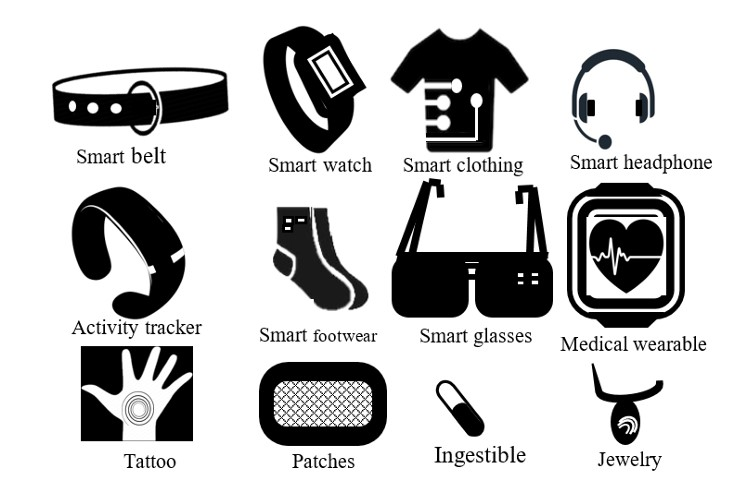
\includegraphics[width=0.55\linewidth]{differentWearables.jpg}
    \caption{Different wearables~\cite{wearablesAndIOT}.}
    \label{fig:difWearables}
\end{figure}

Nowadays there are many different wearables that can collect the same type of data. With this in mind, the choice for the right device doesn't only revolve around what type of information 
it can collect. Portability, processing power, accessibility, battery life are some other important characteristics.


\subsection{Applications}
\label{sub:aplications}

Wearables provide data useful for many applications. Their portability, affordability, easy connection to a mobile phone and non-prescription nature of these devices
 makes them an easy choice for several uses. Amongst others the main ones are Health, Activity Recognition and Sports and Tracking/Localization~\cite{wearablesAndIOT}. 

\subsubsection{Health}
\label{ssub:health}

In the health sector wearables have gained a lot of importance over the last few years. With smart devices, doctors and patients can get a continuous health monitoring which lead to better diagnostics and disease and injury prevention. 
The data provided by the devices is also used to design insoles, shoes and other objects that aid health care and injury prevention~\cite{injuryWalking}.
Besides this, wearables are also being used by people to track their own health without any prescription. 

Construction companies have also been investing in wearables to prevent injuries in their staff when working with heavy loads. In 2020 there were 619 million people affected by lower 
back pain globally and the number is estimated to increase to 843 million by 2050~\cite{lowerBack}.


\subsubsection{Tracking and Localization}
\label{ssub:trackingAndLocalization}

Knowing the position of a person or an animal is important in many occasions. From tracking animals to understand their behaviour to simply finding where a lost elder is, this category has many useful applications.

This devices tend to have a great battery life efficiency since they have to last long periods of time without being charged. 

\subsubsection{Activity Recognition and Sports}
\label{ssub:activityRecognitionAndSports}

Even tho this section has a lot of overlapping technology with the health segment, its use cases go beyond the health category. Besides the day-to-day monitoring these devices can also recognize and monitor your physical activities.

With information about timings, amount of force, position and others, coaches and players can prevent injuries and improve their skills.

\subsubsection{Others}
\label{ssub:others}

Wearables are also used for education, gaming, virtual and augmented reality, law enforcement besides other applications.

\newpage

\subsection{Wearables in Basketball}
\label{sub:wearablesInBasketball}

Basketball was created in 1891 by a Canadian physical education professor named James Naismith in Springfield, Massachusetts as an indoor game to avoid the rain. 

Sensors initially became part of the game through the ball manufacturing process in the 1950s to improve safety and standardization of its pressure. In the 1980s the players started 
using blood oxygen and hear rate monitors in their training to improve strength and conditioning. The development of image sensors led to the recording and live broadcasting of basketball 
games in the 1990s and the 2000s. Displacement and acceleration sensors starting being used in the 2010s to monitor the players' shooting form and other movements. As mentioned in \autoref{sec:wearables} 
wearable technology is rapidly evolving and it is the next big step for sports statistics and performance improvement.~\cite{perspective}.

\begin{figure}[htbp]
    \centering
    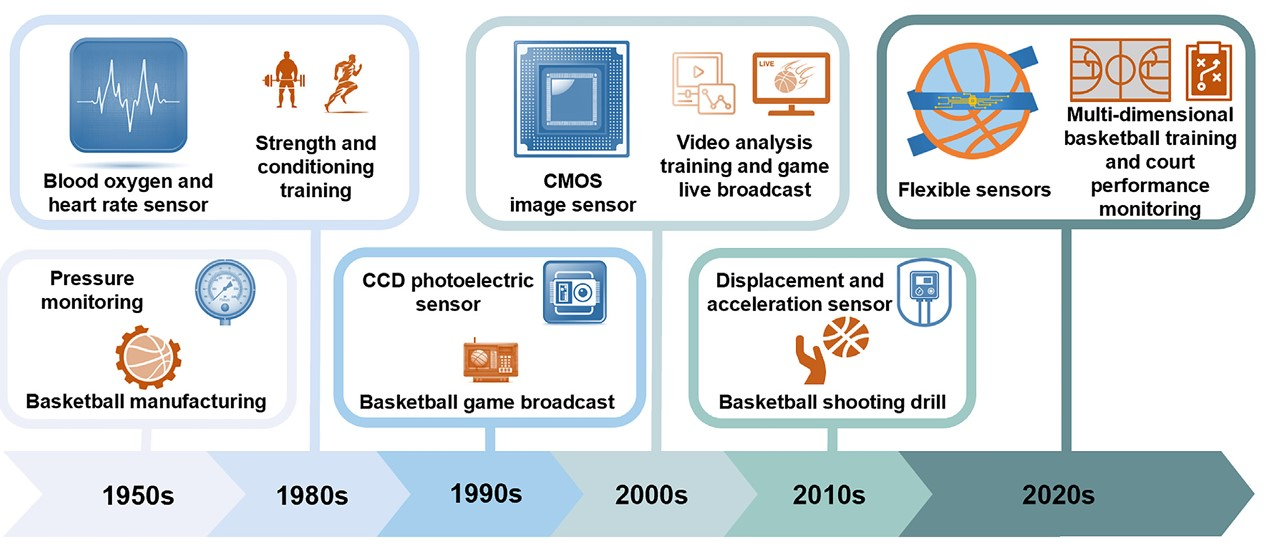
\includegraphics[width=0.8\linewidth]{timeline.jpg}
    \caption{~\cite[Timeline of sensing technology intertwined with basketball sport]{perspective}.}
    \label{fig:sensorTimeline}
\end{figure}

Dave Brailsford popularized the concept "Marginal gains" which consists in improving every single detail, no matter how small in order to get get better. The biggest obstacle in 
this philosophy is quantifying and identifying what we can improve. The answer to this distress are Wearables~\cite{impactWearable}.

For this purpose the technology used consists mostly of micro-electromechanical systems such as inertial measurement units (IMU's), networked sensor suites and exoskeletons. 
Risk assessment shares some of its data with performance enhancement devices but it also works with 
pressure sensors and IMU's that host several sensors (e.g., accelerometers, gyroscopes, and magnetometers)~\cite{biomechanicalPerfomance}. 

\section{Project Introduction}
\label{sec:introduction}

When comparing team sports to single-activity recognition, due to the involvement of two parties trying to better the other one and its unpredictability, team sports have a greater complexity. 
They also involve a lot of high intensity short periods of time and stress, induced by some game situations specially at game climax~\cite{performanceAndTactics}. 

For basketball in particular, the movements consist in a lot of short sprints, quick changes of pace and direction, lateral movement and high jumps (vertical and horizontal) and its high tense moments are more common 
at the end of games (fourth quarter), specially at the last minutes.

Basketball and more specifically, the NBA are becoming more popular globally with each passing year. This leads to more data and more efficient ways to capture it. The most common method 
of doing it is through video recording but these devices are expensive and only the teams with high budgets can afford them~\cite{basketballMotions}. 
The NBA collects statistics through several high definition 3D cameras than can record the whole field. This technology is called SportVU and has been introduced to the league in September of 2013~\cite{basketballFootwork}.

For this project two devices consisting of an Arduino and an Emg Sensor will be used to collect data. This is an initial design that can be improved by implementing these sensors into an 
insole or a sock making it as comfortable and as unnoticeable as possible. An android application will be developed as an interface for the user and the database used.

This project will be based on a prototype of a smart insole designed beforehand. This device has several pressure sensors and an IMU that will be used to identify different basketball 
movements and determine if they're injury prone or not\cite{masterInsole, bachelorInsole}.
Even tho another device would increased precision and add more types of data, in basketball, the only allowed wearables are the ones that can be hidden and won't cause any disturbances 
or interferences in the game such as injuring someone. 

%TO DO - IMU

